% neuer Zeitslot
\newcommand{\talktime}{9:99}
\newcommand{\newtimeslot}[1]{\newpage\renewcommand{\talktime}{#1}}

% neuer Zeitslot ohne Seitenumbruch
\newcommand{\newsmalltimeslot}[1]{\renewcommand{\talktime}{#1}}

% \konferenztag initialisieren
\newcommand{\konferenztag}{KeinTag}


% Standard-Seitenstil definieren (Schnittmarken mit Seitenazhl)
\DeclareNewLayer[background, oddorevenpage, width=125mm,%
height=169mm, contents={%
  
\includegraphics{wallpaper/crop-marks.pdf}%
}]{cropmarksevery}
\newpairofpagestyles[scrheadings]{cropmarksstyle}{}
\AddLayersAtBeginOfPageStyle{cropmarksstyle}{cropmarksevery}

% Seitenstil für Titelseite
\DeclareNewLayer[background, oddorevenpage, width=125mm,%
height=169mm, contents={%
  
\includegraphics{wallpaper/deckseite-vektor-mit-schnittmarken.pdf}%
}]{titlelayer}
\newpairofpagestyles[]{titlestyle}{}
\AddLayersAtBeginOfPageStyle{titlestyle}{titlelayer}

% Hintergrund setzen
\def\mittwoch{Mittwoch}
\def\donnerstag{Donnerstag}
\def\freitag{Freitag}

% Seitenstile definieren
% Mittwoch
\DeclareNewLayer[background, oddpage,  width=125mm,%
height=169mm, contents={%
  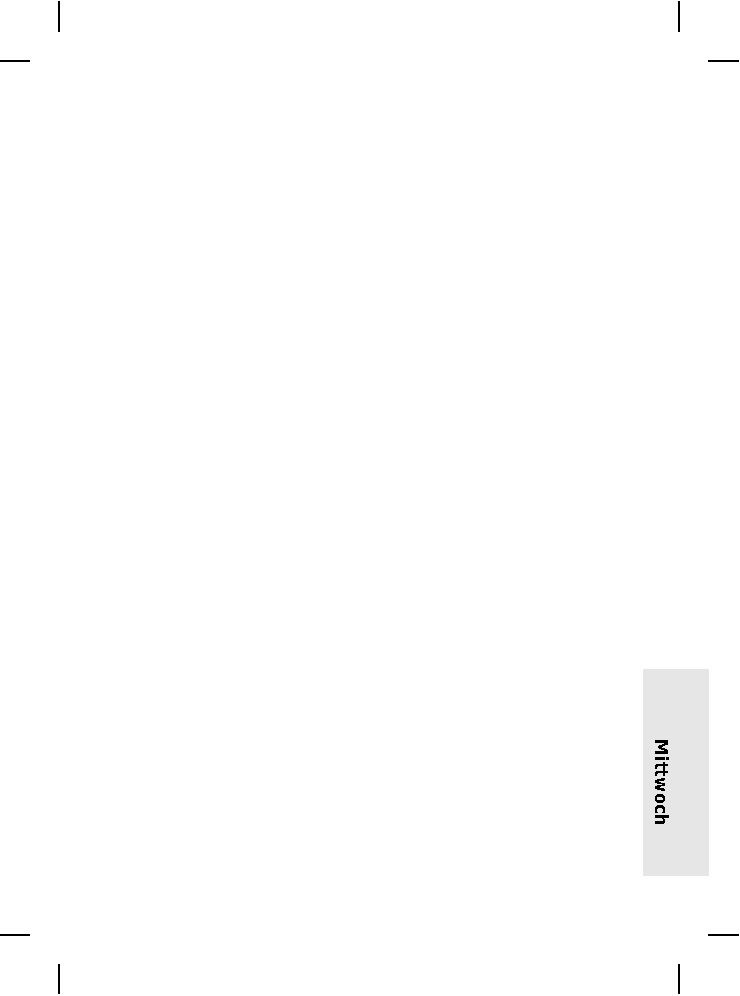
\includegraphics{wallpaper/mittwoch-ungerade.pdf}%
}]{mittwochungerade}
\DeclareNewLayer[background, evenpage,  width=125mm,%
height=169mm, contents={%
  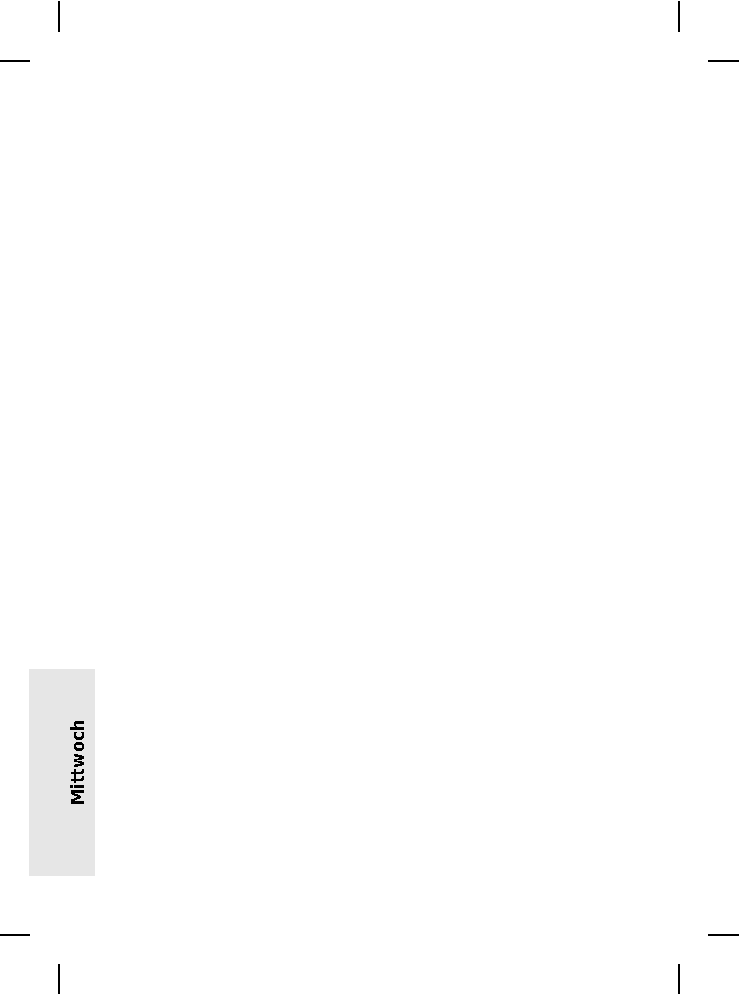
\includegraphics{wallpaper/mittwoch-gerade.pdf}%
}]{mittwochgerade}
\newpairofpagestyles[scrheadings]{mittwoch}{}
\AddLayersAtBeginOfPageStyle{mittwoch}{mittwochgerade}
\AddLayersAtBeginOfPageStyle{mittwoch}{mittwochungerade}
% Donnerstag
\DeclareNewLayer[background, oddpage,  width=125mm,%
height=169mm, contents={%
  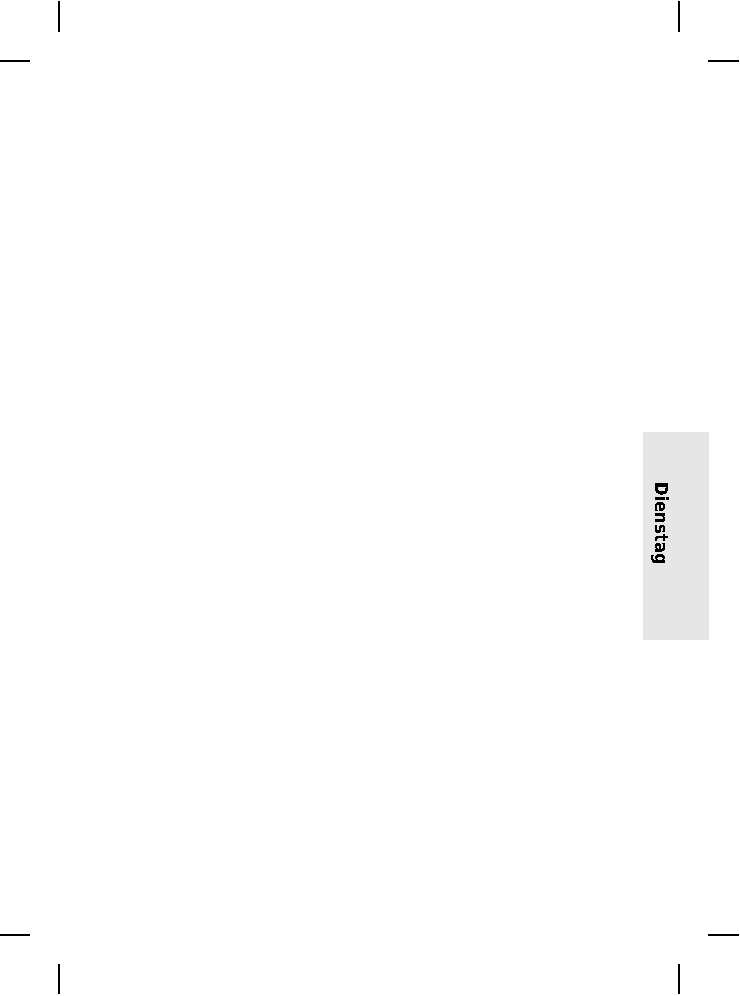
\includegraphics{wallpaper/donnerstag-ungerade.pdf}%
}]{donnerstagungerade}
\DeclareNewLayer[background, evenpage,  width=125mm,%
height=169mm, contents={%
  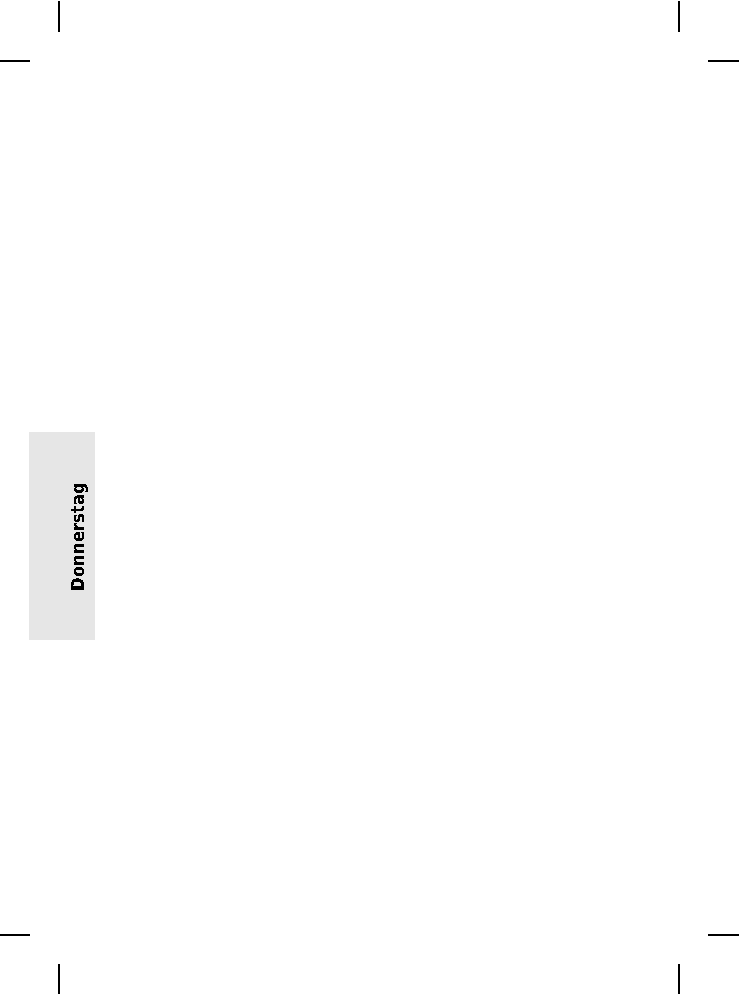
\includegraphics{wallpaper/donnerstag-gerade.pdf}%
}]{donnerstaggerade}
\DeclareNewLayer[background, oddpage,  width=125mm,%
height=169mm, contents={%
  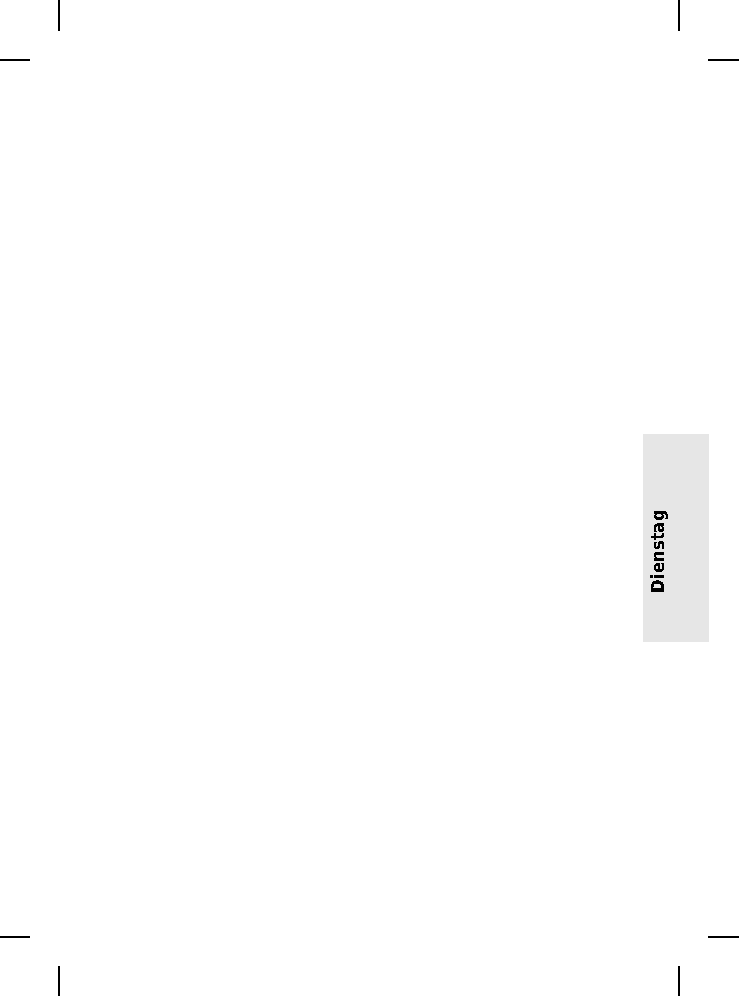
\includegraphics{wallpaper/donnerstag-ungerade-gedreht.pdf}%
}]{donnerstagungeradegedreht}
\newpairofpagestyles[scrheadings]{donnerstag-tabelle}{}
\AddLayersAtBeginOfPageStyle{donnerstag-tabelle}{donnerstaggerade}
\AddLayersAtBeginOfPageStyle{donnerstag-tabelle}{donnerstagungeradegedreht}
\newpairofpagestyles[scrheadings]{donnerstag}{}
\AddLayersAtBeginOfPageStyle{donnerstag}{donnerstaggerade}
\AddLayersAtBeginOfPageStyle{donnerstag}{donnerstagungerade}
% Freitag
\DeclareNewLayer[background, oddpage,  width=125mm,%
height=169mm, contents={%
  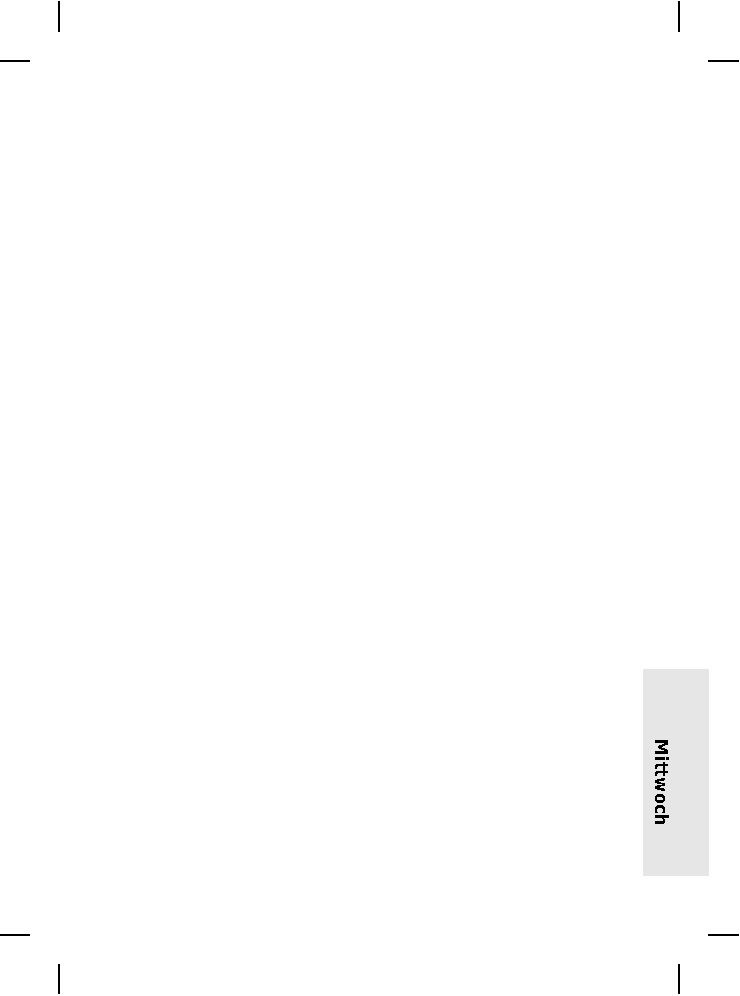
\includegraphics{wallpaper/freitag-ungerade.pdf}%
}]{freitagungerade}
\DeclareNewLayer[background, evenpage,  width=125mm,%
height=169mm, contents={%
  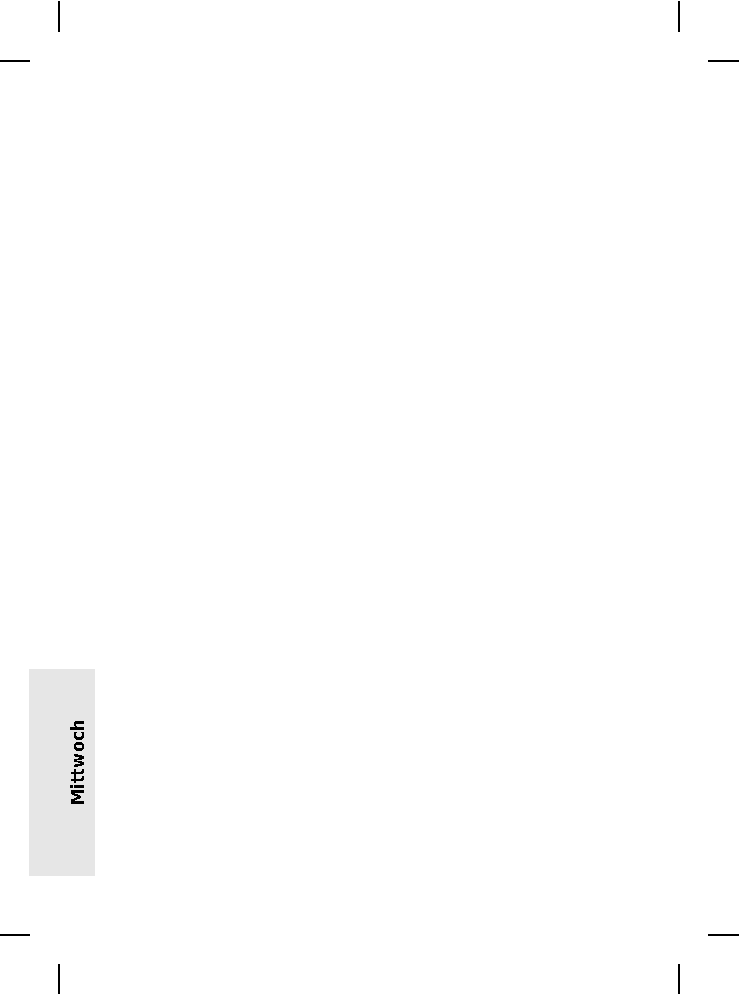
\includegraphics{wallpaper/freitag-gerade.pdf}%
}]{freitaggerade}
\newpairofpagestyles[scrheadings]{freitag}{}
\AddLayersAtBeginOfPageStyle{freitag}{freitaggerade}
\AddLayersAtBeginOfPageStyle{freitag}{freitagungerade}

% \setpagebackground wählt anhand des aktuellen Tages aus, welcher
% Seitenstil verwendet werden soll. Jeder Tag ist ein eigener Seitenstil.
\newcommand{\setpagebackground}{ %
  \ifthenelse{\equal{\konferenztag}{\mittwoch}}{%
    \pagestyle{mittwoch}
  }{}
  \ifthenelse{\equal{\konferenztag}{\donnerstag}}{%
    \pagestyle{donnerstag}
  }{}
  \ifthenelse{\equal{\konferenztag}{\freitag}}{%
    \pagestyle{freitag}
  }{}
}


% zusätzlicher Spaltentyp für die Titeltabelle
\newcolumntype{Y}[1]{>{\RaggedRight\arraybackslash}p{#1}}

%% Längen für Titelboxen
\newlength{\titleboxwidth}
\setlength{\titleboxwidth}{\textwidth}
\advance\titleboxwidth by -6pt

% Befehl zum Setzen von Titelboxen
\newcommand{\setabstract}[6]{
	% 1. Sprecher
	% 2. Titel
	% 3. Untertitel
	% 4. Abstract (Text)
	% 5. Farbe
	% 6. Raum
	%\thispagestyle{scrheadings}
  \setpagebackground
	\setlength\tabcolsep{0pt}
	% \setlength{\fboxsep}{0pt}
	\noindent\fcolorbox{white}{#5}{\parbox{\titleboxwidth}{%
		\noindent\begin{tabu}{X[5L]r}
			\isspeakerempty{#1}{#2}{#6}
			\issubtitleempty{#3}
		\end{tabu}%
	}}
	%
	\isabstractempty{#4}%
	\vspace{0.5em}% Abstand zum nächsten Talk, auch wenn es keinen Abstract gibt
	\setlength\tabcolsep{6pt} % Spaltenpadding wieder auf Default setzen
}

% Setzen des Referenten, falls vorhanden
% Wir gehen davon aus, dass es einen Untertitel nur dann gibt, wenn es auch einen Referenten gibt
\makeatletter
\newcommand{\isspeakerempty}[3]{%
	% Arguments:
	% 1. speaker
	% 2. title
	% 3. room
	\@ifmtarg{#1}{%
			\par\noindent\large \sectfont #2% % Titel
			&
			#3, \talktime
			\tabularnewline
		}
		{
			\emph{#1} % Sprecher
			&
			\talktime
			\tabularnewline
			{\par\noindent\large \sectfont #2}% % Titel
			&
			#3
			\tabularnewline
		}
		
}
\makeatother

% Setzen des Untertitels
% muss ausgelagert und durch \makeatletter umgeben sein
\makeatletter
\newcommand{\issubtitleempty}[1]{%
	\@ifnotmtarg{#1}{\multicolumn{2}{Y{\linewidth}}{\vspace{-0.6em} \noindent\bfseries \normalsize \sectfont #1}\tabularnewline}
}
\makeatother

% Setzen des Abstracts, falls vorhanden
% muss ausgelagert und durch \makeatletter umgeben sein
\makeatletter
\newcommand{\isabstractempty}[1]{%
		\vspace{0.5em}\newline%
		#1 \par% % Abstract
		\vspace{1.5em}% Abstand zum nächsten Talk, auch wenn es einen Abstract gibt
}
\makeatother

% Farben definieren
%\definecolor{eins}{cmyk}{ 0 .18 .06 .10}
\definecolor{eins}{cmyk}{ 0 .13 .04 .08}
\definecolor{zwei}{cmyk}{ .1 0 .17 .05}
\definecolor{hellorange}{cmyk}{ 0 0.13 0.35 0.03}
%\definecolor{aula}{cmyk}{ 0.2 0 0.05 0.13}
\definecolor{aula}{cmyk}{ 0.13 0 0.04 0.11}
\definecolor{geoblau}{cmyk}{ 0.2 .02 0 .01}
\definecolor{dezentrot}{cmyk}{ 0 .17 0.21 .04}
\definecolor{hellgelb}{cmyk}{ 0 .02 0.26 0}
\definecolor{hellgruen}{cmyk}{ 0.05 .0 0.17 0.05}

% Abstract AM HS 9
\newcommand{\abstractNeun}[4]%
{%
	\setabstract{#1}{#2}{#3}{#4}{hellgruen}{AM HS\,9}
}

% Abstract IM HS 13
\newcommand{\abstractDreizehn}[4]%
{%
	\setabstract{#1}{#2}{#3}{#4}{hellgelb}{IM HS\,13}
}

% Abstract IM HS 11
\newcommand{\abstractElf}[4]%
{%
	\setabstract{#1}{#2}{#3}{#4}{geoblau}{IM HS\,11}
}

% Abstract AM HS 10
\newcommand{\abstractZehn}[4]%
{%
	\setabstract{#1}{#2}{#3}{#4}{hellorange}{AM HS\,10}
}

% Workshop STUDLAB
\newcommand{\workshopbox}[3]%
{%
	% 1. Titel
	% 2. Referent
	% 3. HS-Nummer
	\setlength\tabcolsep{0pt}
	\noindent\fcolorbox{white}{dezentrot}{\parbox{\titleboxwidth}{%
			\noindent
			\begin{tabu}{X[5L]r}
				\emph{#2} % Sprecher
				&
				\talktime
				\tabularnewline
				{\noindent\large \bfseries #1}% % Titel
				&
				Workshop #3
				\tabularnewline
			\end{tabu}
		}
	}
	\setlength\tabcolsep{6pt} % Spaltenpadding wieder auf Default setzen
}

% viel zu lang
\newcommand{\zulang}{Dieser Text ist viel zu lang. Dieser Text ist viel zu lang. Dieser Text ist viel zu lang. Dieser Text ist viel zu lang. Dieser Text ist viel zu lang. Dieser Text ist viel zu lang. Dieser Text ist viel zu lang. Dieser Text ist viel zu lang. Dieser Text ist viel zu lang. Dieser Text ist viel zu lang. Dieser Text ist viel zu lang. Dieser Text ist viel zu lang. Dieser Text ist viel zu lang. Dieser Text ist viel zu lang. }

%% Längen für Sponsorenbox
\newlength{\fboxwidth}

\def\workshopsSection{workshopsSection}
\def\abstractsSection{abstractsSection}
\newcommand{\sponsorenbox}[4]{%
  %% Längen für Sponsorenbox
  \setlength{\fboxwidth}{\textwidth}
  \advance\fboxwidth by -7.0pt
  \abstractSponsorenbox{#1}{#2}{#3}{#4}{\workshopsSection}%
}

\newcommand{\sponsorenboxA}[4]{%
  %% Längen für Sponsorenbox
  \setlength{\fboxwidth}{\textwidth}
  \advance\fboxwidth by -10.0pt
  \abstractSponsorenbox{#1}{#2}{#3}{#4}{\abstractsSection}%
}

%% Sponsorenbox
%% 1. Logo
%% 2. Logobreite
%% 3. Anzahl benötigter Zeilen
%% 4. Text
%% 5. Umfeld (\workshopsSection oder \abstractsSection}
\makeatletter
\newcommand{\abstractSponsorenbox}[5]{%
  \setlength{\fboxsep}{4.5pt}%
  \noindent%
  \ifthenelse{\equal{#5}{\workshopsSection}}{%
    \hspace{2.65pt}%
  }{\hspace{-1pt}}%
  \fcolorbox{gray}{white}{\parbox{\fboxwidth}{
    \@ifmtarg{#1}{}{%
      \begin{wrapfigure}[#3]{r}[0pt]{#2}
        \centering\vspace{-1\baselineskip}
        \includegraphics[width=#2]{#1}
      \end{wrapfigure}
    }

    \noindent #4
  }}
  \setlength{\fboxsep}{3pt}
}
\makeatother

% Definitionen für Tagestabellen
\newcolumntype{Z}[1]{>{\RaggedRight\arraybackslash}p{#1}}%
\newcolumntype{C}[1]{>{\Centering\arraybackslash}p{#1}}%
\newcommand{\talk}[2]%
{%
	& \textbf{#1} \newline \emph{#2}
}%
% Titel -- Redner


\newcommand{\workshop}[3]%
{%
	\workshopbox{#1}{#2}{#3}
}%

\newcommand{\otherevent}[1]%
{%
	& \textbf{#1}
}%

\newcommand{\aulaevent}[2]%
{%
	&
	\multicolumn{3}{c}{
		\textbf{#1} (Aula) \par \emph{#2}
	}
}%

\newcommand{\coffeespace}{\vspace{0.4em}}
\newcommand{\workshopspace}{\vspace{0.5em}\\}

% Farben definieren
\definecolor{commongray}{gray}{.9}
%\vspace{-1.2em}
\renewcommand{\arraystretch}{1.4}
